% vim: set fenc=utf-8 ft=latex encoding=utf-8
% -*- mode: latex; coding: UTF-8; -*-
%!TEX root = knowledge-curation.tex
\section{Introduction}
\label{cha:introduction}

\dmg{Intro is 1 paragraph too long (make it all fit in one page)}

    % Software development today
    Today's software development is more about just-in-time learning than reading manuals~\cite{Hartmann2008}.
    With instantaneous access to information on the Web, programmers do not have to be experts in a particular technology to build an application.
    Programmers can consult a variety of online resources, such as Stack Overflow\footnote{\url{http://stackoverflow.com/}}, by entering combinations of keywords in a search engine.
    If they cannot find the correct answer there are many easy-to-use \textit{media channels} for assistance, from which they can address most programming problems within minutes or seconds~\cite{Mamykina2011}.

    % Role of media channels
Media channels play an important role in today's knowledge economy, as well as the collaboration, coordination, and communication activities that occur between programmers.
Media channels are more than just delivery systems---they connect users with a \textit{community of practice} or groups of people with a common interest.
Selecting the most appropriate media channel to transmit an idea can be challenging, given the variety of equally suitable tools and sites.
To decide, a programmer considers the characteristics will benefit most among channels.
Such considerations are: experts on the channel, flexibility on topics allowed, if the channel is asynchronous, socially enabled, or has gamification elements~\cite{Vasilescu2014c}.

    % Media channels connect communities
%   Each community has its own implicit or explicit norms.
%   Any violation of the community norms or channel rules may result in unfriendly responses from the community, or being flagged with a bad reputation.
%   Depending on the media channel, a bad online reputation can affect real life events.
%   For instance, Singer \textit{et al}. found that reputation on Stack Overflow is used by recruiters to assess programmer performance~\cite{Singer2013}.

%This investigation is motivated by an open challenge presented by Vasilescu~\cite{Vasilescu2014b}, that states \textit{``...to better understand the effects associated with a transition from mailing lists to social Q\&A and, e.g., whether mailing lists will eventually die off, future research could also consider analysing the content of the discussions from the two venues...''}.
%This challenge raised a desire to understand the knowledge flow through channels that serve the same purpose.

    We investigated the way \textit{knowledge} (or user generated content) is curated within a particular software development community.
    For this study we chose the R community, since it provided broader relevance outside the software development community by including users with no or limited programming experience (e.g., biologist or statisticians).
    Our overarching goal was to provide tools for further studies that analyse and compare the knowledge flowing through media channels.
    Thus, the research question investigated are:

\dmg{what about Rephrasing RQ to stress differences between channels also?}
    \begin{enumerate}[label=\bfseries{RQ-\arabic*.},itemsep=3pt, topsep=2pt, leftmargin=3em, parsep=0pt]
        \item What types of knowledge are shared on Stack Overflow and the R-help mailing list within the R community?
        \item How is the knowledge constructed on Stack Overflow and the R-help mailing list? 
%       \item How does the sharing of links on Stack Overflow and the R-help mailing list support knowledge construction?
        \item Why do certain users post to both Stack Overflow and the R-help mailing list?
    \end{enumerate}

We analysed the main Q\&A channels related to programming that the R community contains: R-help mailing list and Stack Overlow.
To analyse the channels, we applied a qualitative \textit{exploratory case study} methodology.
We also conducted a survey to bring further insights on the findings.
We constructed a series of categories that supports knowledge classification and knowledge comparison of the main type of messages which these two channels provided.
Based on the knowledge categories analysis, we compared the way knowledge was shared on Stack Overflow and the R-help mailing list.
Finally, we extracted a set of recommendations to assist in the usage of multiple Q\&A channels, and when linking resources that are external to both channels.

\dmg{Add a summary of the results}
%\subsection{Contributions}

%   The contributions of this paper are:
%       a comparison of how knowledge is shared on the two channels,
%       I compared the way knowledge is shared on both channels based on the findings of this thesis and the survey data.
%       My objective was to identify the differences of how knowledge is shared on Stack Overflow and the R-help mailing list.
%       a categorization of messages on Q\&A media channels, and
%       I built a categorization of knowledge based on the analysis of data that flows through media channels. 
%       My objective was that categories should support further studies when comparing media channels based on the knowledge flowing through them.
%       With these categorizations I gained insights about knowledge that flows through the channels, and the differences between them.
%        a set of recommendations for using multiple Q\&A media channels.
%       I created and provided a set of recommendations for using multiple media channels based on the observation and analysis of the data.
%       It is meant to improve multiple media channel usage by providing a best practices reference.    
%       and a tool to extract information from mailing lists.
%       Mailing list repositories such as R-help contain valuable information about user behaviours, best practices, topics, problems, and discussions.
%       However, such information exists as unstructured data that needs special processing before it can be studied.
%       To that end, I developed GTMail\footnote{This tool is available online \url{https://github.com/cagomezt/GTMail}.}, a software tool capable of dealing with multiple standardization issues when presented on mailing list data (e.g., duplicates, text formatting), extracting URLs embedded in email bodies, eliminating unnecessary information, and uploading the data to a database for further analysis.
%       My tool is compatible with MBOX mailing list formats, and therefore, can be used in any other research that involves mailing list repositories.

%   \begin{figure}[!htb]
%       \centering
%       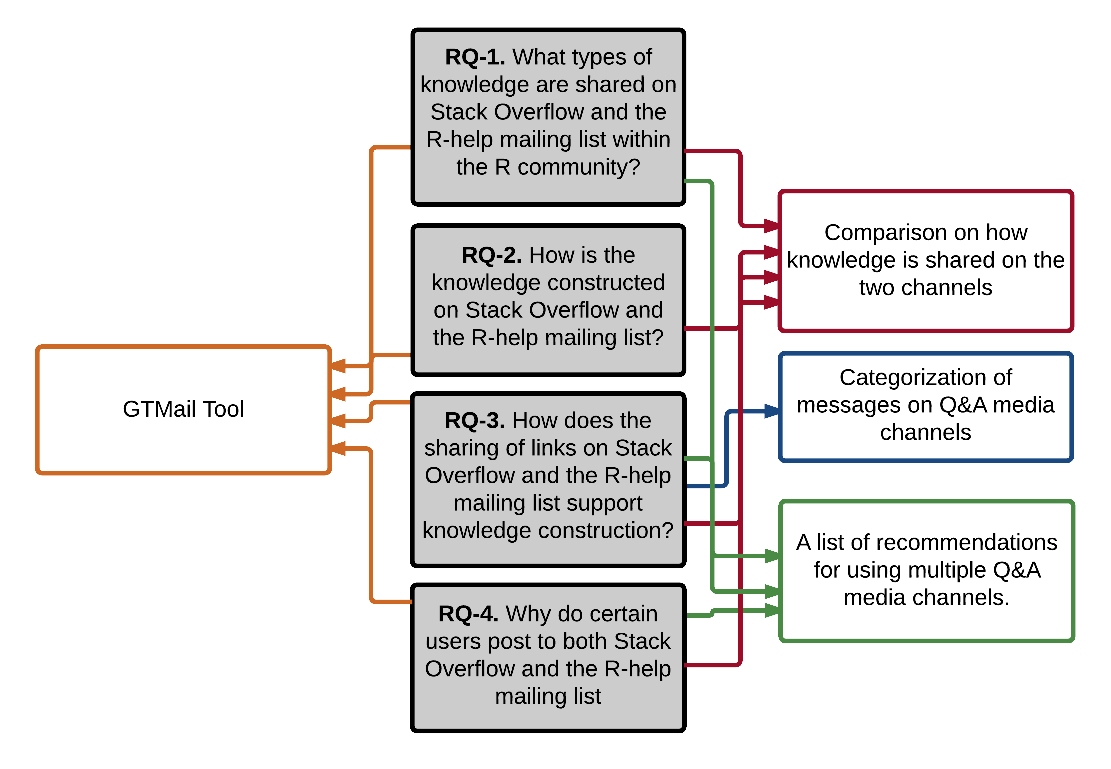
\includegraphics[width=1\columnwidth]{Figures/RQ-contributions}
%       \caption{Mapping between the research questions in this thesis and the contributions.}
%       \label{fig:RQ-contributions}
%   \end{figure}

%   Figure \ref{fig:RQ-contributions} depicts the mapping between my research questions and my contributions. 
%   In the figure, GTMail tool is mapped with all research questions because the tool processes the data used in this thesis.

%%% Local Variables:
%%% mode: latex
%%% TeX-master: "knowledge-curation.tex"
%%% End:
